
\begin{figure}[tbh]
\centerline{
%%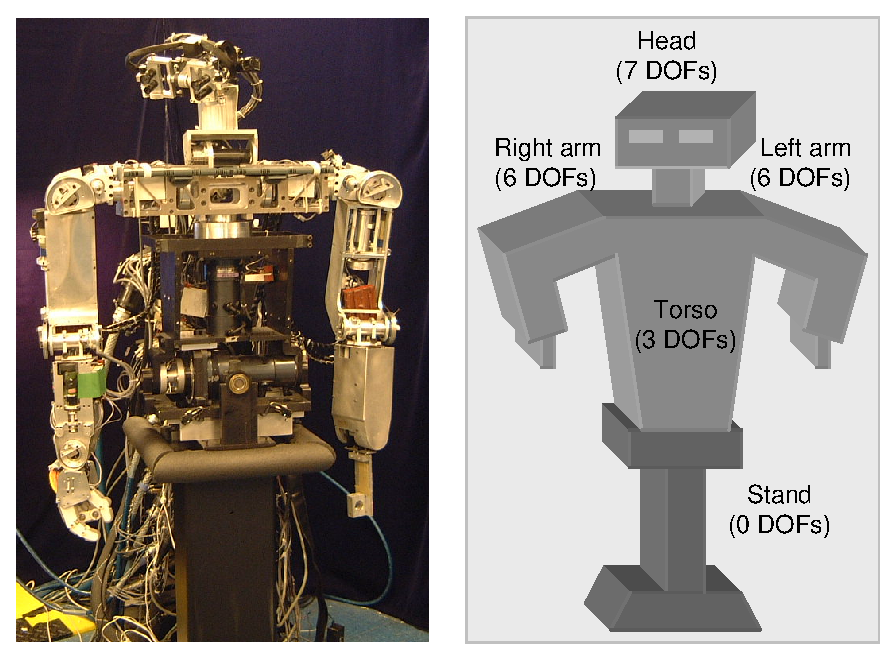
\includegraphics[width=\columnwidth]{cog-schematic.eps}
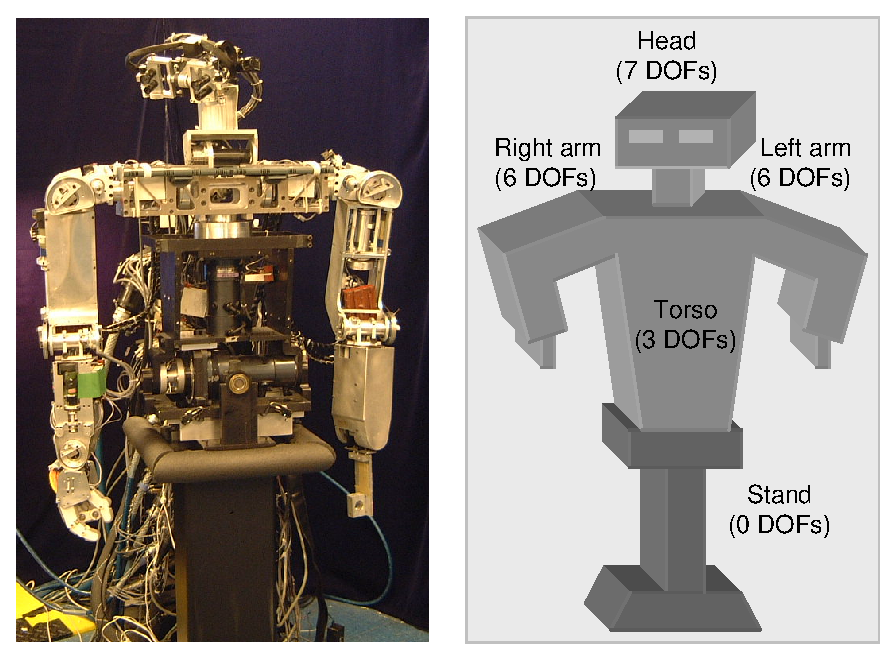
\includegraphics[width=6.0cm]{cog-schematic.eps}
%%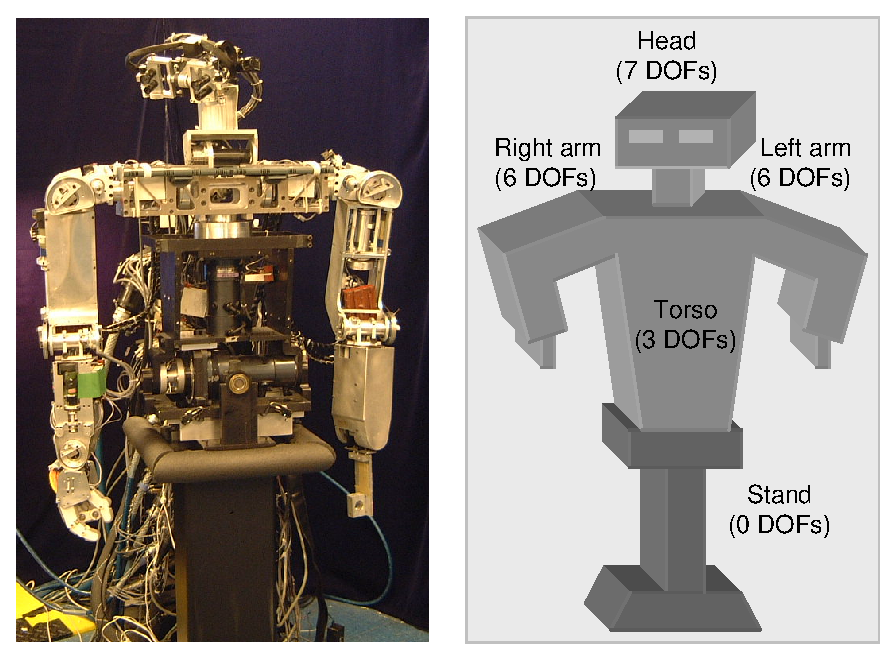
\psfig{file=cog-schematic.eps,height=2.5in,clip=,silent=}
}
\caption{ 
%
  Degrees of freedom (DOFs) of the robot Cog.  The arms terminate
  either in a primitive ``flipper'' or a four-fingered hand.  
\ifverbose
The hand
  is an independent research project by Matthew Marjanovi\'{c}, and
  will not be employed or described here.  
\fi
  The head, torso, and arms
  together contain 22 degrees of freedom.
%
}
\label{fig:cog-schematic}
\end{figure}

\section{Our experimental platform}



\ifverbose
%
\begin{figure}[tbh]
\begin{center}
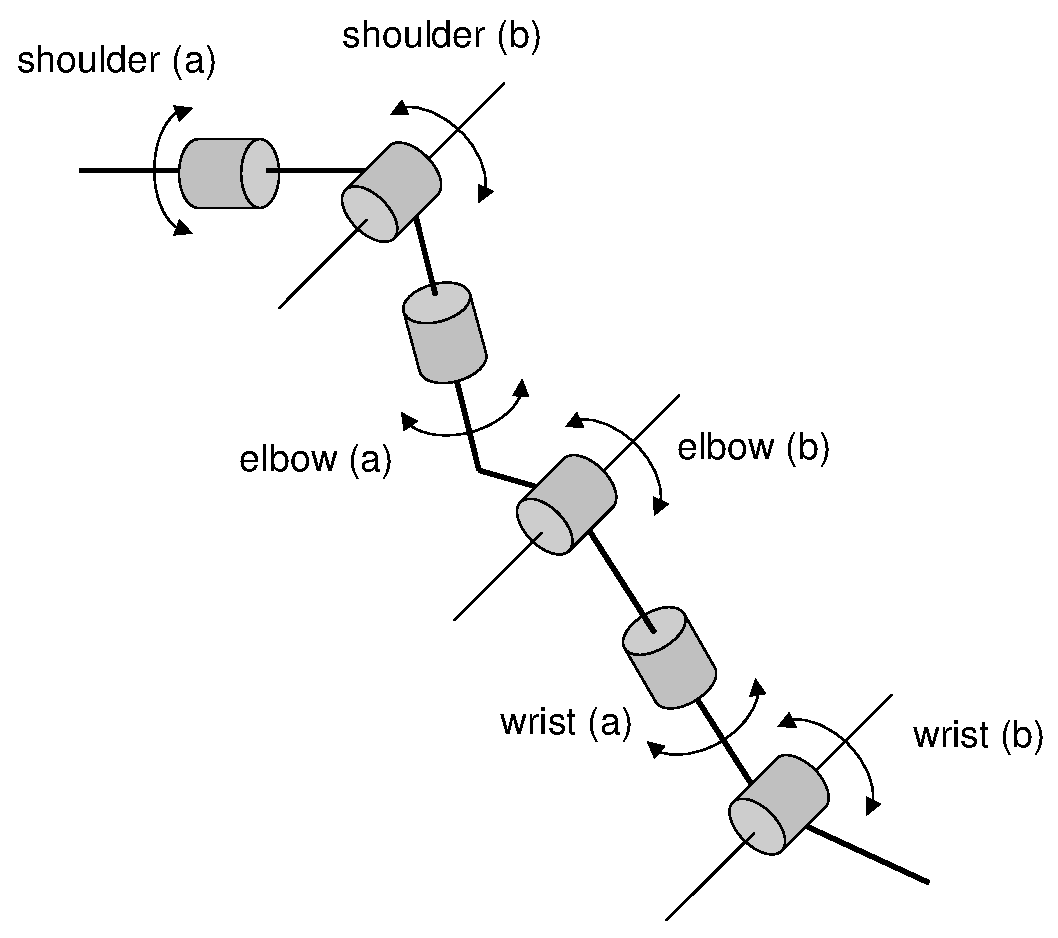
\includegraphics[width=5.0cm]{arm-motors.eps}
\caption{ 
\label{fig:arm-motors}
%
Kinematics of the arm, following \protect\cite{williamson99robot}.
There are a total of six joints, divided into a pair for each of
the shoulder, elbow, and wrist/flipper.
%
}
\end{center}
\end{figure}
%
\fi

This work is implemented on the robot Cog, an upper torso humanoid
\cite{brooks99cog}.  
%%The robot has previously been applied to tasks
%%such as visually-guided pointing \cite{Marjanovic-96-SAB}, and
%%rhythmic operations such as turning a crank or driving a slinky
%%\cite{williamson98neural}.  
Cog has two arms, each of which has six
degrees of freedom. %% -- two per shoulder, elbow, and wrist.
%% (see Figure~\ref{fig:arm-motors}).  
The joints are driven by series elastic
actuators \cite{williamson99robot}.
%% -- essentially a motor connected
%%to its load via a spring (think strong and torsional rather than
%%loosely coiled).  
The arm is not designed to enact trajectories with
high fidelity.  For that a very stiff arm is preferable.  Rather, it
is designed to perform well when interacting with a poorly
characterized environment, where collisions are frequent and
informative events.
Cog runs an attentional system consisting of a set of pre-attentive
filters sensitive to motion, \ahhcolor{}, and binocular disparity. The
different filters generate information on the likelihood that
something interesting is happening in a certain region of the image. A
voting mechanism is used to ``decide'' what to attend and track
next. The pre-attentive filters are implemented on a space-variant
imaging system, which mimics the distribution
of photoreceptors in the human retina.
 The attentional system uses vision and non-visual sensors
(e.g. inertial) to generate a range of oculomotor \ahhbehavior{}s. Examples
are saccades, smooth pursuit, vergence, and the vestibulo-ocular
reflex (VOR).






